\begin{surferIntroPage}{Surfaces Records}{record_chmutovoktic}{Surfaces Records}
    Une surface est \emph{non-singulière} ou \emph{lisse} si elle n'a pas de pointes (ces points sont appelés \emph{singularités}). La sphère et le tore sont deux exemples de surfaces lisses, voir les 2 premières
    images ci-dessous.  
    En général, une surface choisie au hasard est lisse. 
 \begin{center}
      \vspace{-0.2cm}
      \begin{tabular}{@{}c@{}c@{}c@{\quad}c@{}c@{}c@{}c@{}}
        \begin{tabular}{@{}c@{}}
          lisse :
        \end{tabular}
        &
        \begin{tabular}{@{}c@{}}
          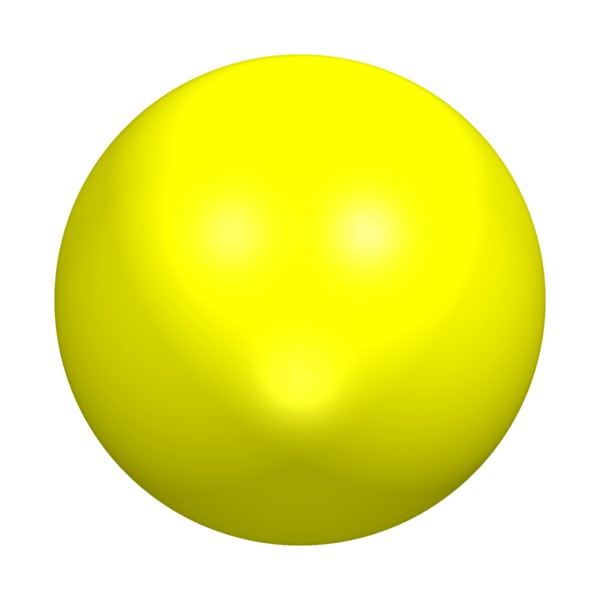
\includegraphics[width=1.1cm]{./../../common/images/kugel}
        \end{tabular}
        &
        \begin{tabular}{@{}c@{}}
          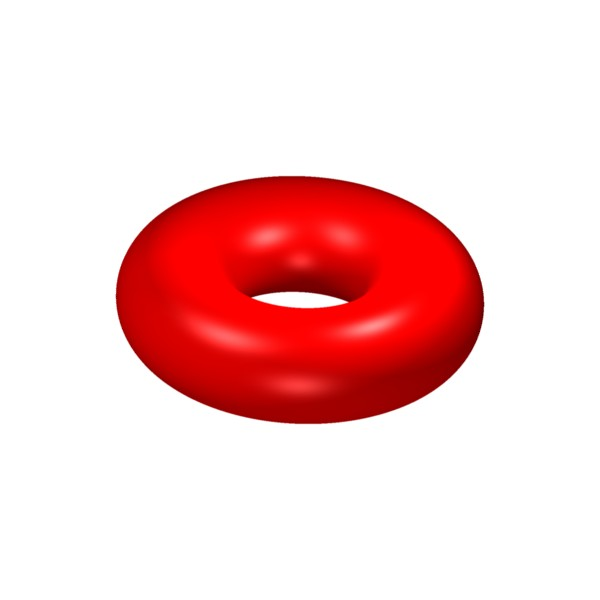
\includegraphics[width=1.1cm]{./../../common/images/torus}
        \end{tabular}
        &
        \begin{tabular}{@{}c@{}}
          nombreuses\\
          singularités:
        \end{tabular}
        &
        \begin{tabular}{c@{}@{}}
          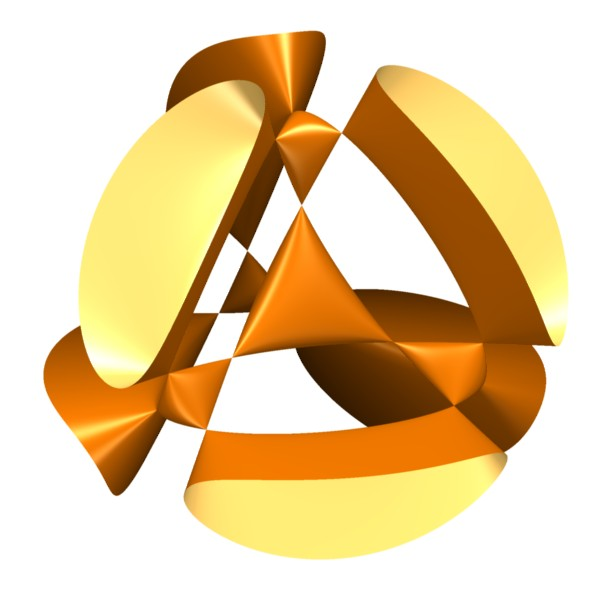
\includegraphics[width=1.1cm]{./../../common/images/kummer}
        \end{tabular}
        &
        \begin{tabular}{c@{}@{}}
          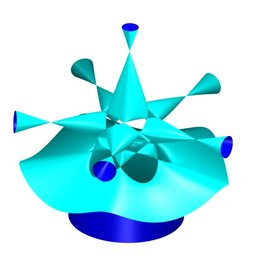
\includegraphics[width=1.1cm]{./../../common/images/togliatti}
        \end{tabular}
        &
        \begin{tabular}{c@{}@{}}
          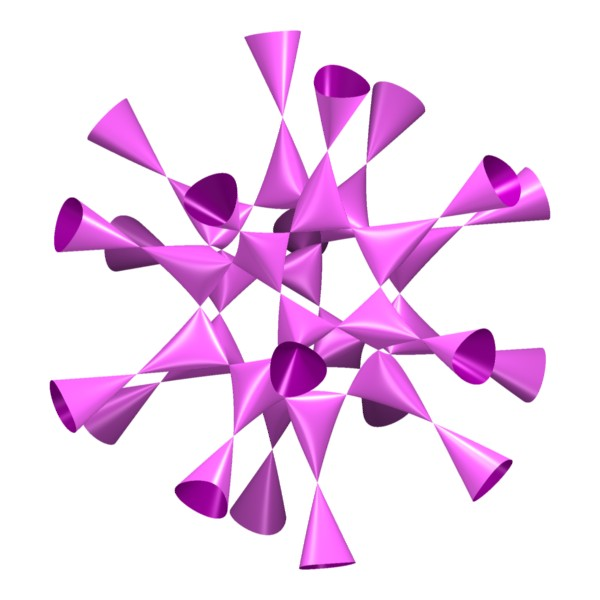
\includegraphics[width=1.1cm]{./../../common/images/barth_sextic}
        \end{tabular}
      \end{tabular}
    \end{center}
    \vspace{-0.2cm}
    Les surfaces exhibant des singularités constituent donc des cas très spéciaux. Ces points sont les plus intéressants d'une surface. Les surfaces du programme SURFER sont définies par les zéros de polynômes, où les variables apparaissent seulement avec des puissances entières positives. La plus grande valeur de la somme des puissances pour chaque terme est le degré, $d$. En mathématiques, on se demande combien de singularités peut avoir une surface de degré $d$ donné.
    On désigne ce nombre par $\mu(d)$. Il apparaît que ce nombre $\mu(d)$ est très difficile à calculer.
    Sa valeur pour $d=1,2,3,4$ est connue depuis le $19$è siècle, alors que sa valeur pour $d=5$
    n'a été trouvée qu'en 1980, et en 1996 pour $d=6$.
    Pour $d\ge 7$, $\mu(d)$ n'est toujours pas connu.
    Chaque nouveau record pour un $\mu(d)$ est donc un résultat partiel important. Cela risque de demander encore beaucoup de temps avant d'avoir une réponse valide pour toute valeur de $d$.\\  Quelques résultats connus :
    
   \begin{center}
      \begin{tabular}{r|cccccccc|c}
        $d$ & $1$ & $2$ & $3$ & $4$ & $5$ & $6$ & $7$ & $8$ & $d$\\
        \hline
        \hline
        \rule{0pt}{1.2em}$\mu(d)\ge$ & $0$ & $1$ & $4$ & $16$ & $31$ & $65$ &
        $99$ & $168$ & 
        $\approx \frac{5}{12}d^3$\\[0.3em]
        \hline
        \rule{0pt}{1.2em}$\mu(d)\le$ & $0$ & $1$ & $4$ & $16$ & $31$ & $65$ &
        $104$ & $174$ & $\approx \frac{4}{9}d^3$
      \end{tabular}
    \end{center}
\end{surferIntroPage}
